% Provenance (never printed): cycle 4 SVT, "La planete Terre, l'environnement
% et l'action humaine": natural risks, hazard and vulnerability, prevention
% and protection; see sources/book1/PROVENANCE.md. Book 1, grade 9, chapter 2.
% Vocabulary guard: owns risk, vulnerability, prevention, hazard map.
% Natural hazard and natural disaster, the warning colours and the safety
% rules are g5's (natural-hazards); the warning signs of an eruption and the
% Pinatubo story are g7's (volcanoes); seismometer, tsunami and "scientists
% cannot predict earthquakes" are g7's (earthquakes); flood and floodplain
% are g5's (water-shapes-the-land); weather forecast is g8's. Lahars are
% called mudflows (as in g7). "Normal fault" is Book 2's: here "a fault".
\chapter{العيش مع المخاطر الطبيعية}\label{ch:g9:natural-risks}

في وقت متأخر من مساء 13~نوفمبر 1985، كان معظم سكان أرميرو، وهي بلدة في
كولومبيا، في أسرّتهم. وكانت \omterm{def:g5:natural-hazards:storm}{عاصفة} تحجب \omterm{def:g4:volcanoes-earthquakes-first-look:volcano}{البركان} المكلل بالثلوج نيفادو ديل رويز،
على بعد \qty{45}{km}، فلم يره أحد في البلدة وهو يثور. وأذابت \omterm{def:g3:stones-pebbles-sand:rock}{الصخور} الحارة جزءًا
من جليده، فاندفع الماء، مختلطًا بالرماد \omterm{def:g3:stones-pebbles-sand:rock}{والصخر}، في \omterm{def:g1:landscapes-around-us:landform}{الأودية} سيولًا طينية. وبعد
نحو ساعتين، خرجت السيول الطينية من \omterm{def:g1:landscapes-around-us:landform}{وادي} \omterm{def:g1:landscapes-around-us:water}{نهر} لاغونياس، واندفعت مباشرة إلى
البلدة: فقُتل نحو \num{23000} شخص، أي معظم سكان البلدة. وكانت ساعتان وقتًا كافيًا
للسير إلى أرض أعلى. لكن أحدًا لم يخبر سكان أرميرو.
% ledger: usgs:armero

\begin{omfigure}
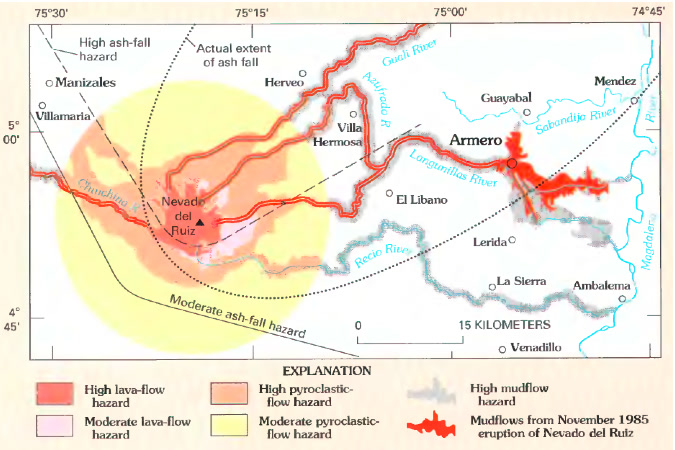
\includegraphics[width=0.86\linewidth]{images/book1/g9-ruiz-hazard-map.jpg}

{\small \omterm{def:g9:natural-risks:hazard-map}{خريطة الأخطار} \omterm{def:g4:volcanoes-earthquakes-first-look:volcano}{لبركان} نيفادو ديل رويز. وُزّعت نسخة أولى منها، رسمها
جيولوجيون كولومبيون، قبل \omterm{def:g4:volcanoes-earthquakes-first-look:eruption}{الثوران} بشهر، وكانت تبين من قبلُ خطر السيول الطينية في
\omterm{def:g1:landscapes-around-us:landform}{وادي} أرميرو. وهذه النسخة، المعاد رسمها بعد الكارثة، تضيف بالأحمر الساطع السيول
الطينية التي جاءت فعلًا في نوفمبر 1985 (يبلغ نصف قطر الدائرة المظللة حول \omterm{def:g4:volcanoes-earthquakes-first-look:volcano}{البركان}
نحو \qty{20}{km}). عن ت.~ل.~رايت وت.~ك.~بيرسون، النشرة 1073 لهيئة المسح الجيولوجي
الأمريكية، 1992 (ملك عام، عبر ويكيميديا كومنز).}
% ledger: usgs:ruiz-map, commons:ruiz-map
\label{fig:g9:natural-risks:ruiz}
\end{omfigure}

بعد ست سنوات، في \omterm{def:g1:landscapes-around-us:landform}{جبل} بيناتوبو في الفلبين، كان \omterm{def:g4:volcanoes-earthquakes-first-look:volcano}{البركان} مراقَبًا، فجاء الإنذار في
وقته وغادر الناس (\cref{ch:g7:volcanoes}). وكان كلاهما \omterm{def:g4:volcanoes-earthquakes-first-look:volcano}{بركانًا} انفجاريًا، يعيش
الناس في طريق سيوله الطينية. أما الفرق فكان في ما عرفه الناس، وفي ما فعلوه بما
عرفوه. وهذا الفصل يدور حول ذلك
الفرق.
% ledger: usgs:armero (Pinatubo 1991 averted a disaster like Armero), usgs:pinatubo-1991

\begin{recall}
\emph{\omterm{def:g5:natural-hazards:hazard}{الخطر الطبيعي}} حدث طبيعي قد يؤذي الناس؛ ويصير \emph{\omterm{def:g5:natural-hazards:disaster}{كارثة طبيعية}} حين يضرب
حيث يعيش الناس ويُلحق ضررًا كبيرًا (\cref{ch:g5:natural-hazards}). \omterm{def:g1:landscapes-around-us:water}{والنهر} الذي
يفيض يغطي \omterm{def:g5:water-shapes-the-land:flood}{سهله الفيضي} (\cref{ch:g5:water-shapes-the-land}). وكثيرًا ما يعطي
\omterm{def:g4:volcanoes-earthquakes-first-look:volcano}{البركان} علامات إنذار قبل \omterm{def:g4:volcanoes-earthquakes-first-look:eruption}{ثوران} كبير: \omterm{def:g4:volcanoes-earthquakes-first-look:earthquake}{زلازل} صغيرة، وانتفاخ المنحدرات، وغازات
(\cref{ch:g7:volcanoes}). ولا يستطيع العلماء التنبؤ \omterm{def:g4:volcanoes-earthquakes-first-look:earthquake}{بالزلازل}؛ \omterm{def:g7:earthquakes:seismometer}{فمقاييس الزلازل}
تسجلها، \omterm{def:g4:volcanoes-earthquakes-first-look:earthquake}{والزلزال} تحت \omterm{def:g2:water-on-earth:ocean}{البحر} قد يطلق \omterm{def:g7:earthquakes:tsunami}{تسونامي} (\cref{ch:g7:earthquakes}). \omterm{def:g8:fronts-and-weather-maps:forecast}{والتنبؤ
بالطقس} يقول كيف سيكون \omterm{def:g1:watching-the-weather:weather}{الطقس} في الأيام القادمة
(\cref{ch:g8:fronts-and-weather-maps}).
\end{recall}

\section{الخطر والهشاشة والمخاطر}

\omterm{def:g4:volcanoes-earthquakes-first-look:earthquake}{الزلزال} نفسه لا يُلحق الضرر نفسه في كل مكان. فتحت \omterm{def:g5:weather-and-climate:desert}{صحراء} خالية لا يؤذي أحدًا.
وتحت مدينة مبانيها متينة ويعرف سكانها ما يفعلون، يهز ويخيف ويكسر النوافذ. وتحت
مدينة بيوتها ثقيلة سيئة البناء، قد يُسقطها على من فيها. فالخطر هو نفسه؛ وما
يتغير هو مدى سهولة تضرر المكان.

\begin{definition}[الهشاشة]\label{def:g9:natural-risks:vulnerability}
\emph{هشاشة}\index{هشاشة} مكان ما هي مدى سهولة تضرر سكانه ومبانيه وما يحتاجون
إليه من \omterm{def:g5:natural-hazards:hazard}{خطر طبيعي}. فالبيوت على \omterm{def:g5:water-shapes-the-land:flood}{سهل فيضي}، والمباني الضعيفة، وغياب الإنذار وغياب
الخطة تجعل المكان هشًّا.
\end{definition}

\begin{definition}[المخاطر]\label{def:g9:natural-risks:risk}
\emph{المخاطر}\index{مخاطر} التي يواجهها مكان ما من \omterm{def:g5:natural-hazards:hazard}{خطر طبيعي} هي احتمال وقوع
الضرر بسكانه وممتلكاتهم. وهي تتوقف على الخطر، أي مدى قوته ومدى تكراره، وعلى
\omterm{def:g9:natural-risks:vulnerability}{هشاشة} المكان معًا: فحيث لا خطر، أو لا شيء يمكن أن يتضرر، لا مخاطر.
\end{definition}

\begin{omfigure}
\begin{tikzpicture}[x=1cm, y=1cm, font=\footnotesize,
    cell/.style={minimum width=4.6cm, minimum height=2.2cm, align=center, draw=black!50, text width=4.2cm}]
  \node[cell, fill=green!25] at (2.3,1.1) {\textbf{مخاطر منخفضة}\\ فيضان صغير في وادٍ\\ لا يسكنه أحد};
  \node[cell, fill=orange!30] at (6.9,1.1) {\textbf{مخاطر متوسطة}\\ زلزال قوي تحت مدينة\\ مبانيها متينة\\ وسكانها مستعدون};
  \node[cell, fill=orange!30] at (2.3,3.3) {\textbf{مخاطر متوسطة}\\ فيضان صغير في قرية\\ مبنية على السهل الفيضي};
  \node[cell, fill=red!35] at (6.9,3.3) {\textbf{مخاطر عالية}\\ زلزال قوي تحت مدينة\\ مبانيها ضعيفة\\ ولا خطة لديها};
  \draw[->, thick] (0,-0.25) -- (9.4,-0.25);
  \draw[->, thick] (-0.25,0) -- (-0.25,4.6);
  \node[anchor=north] at (4.6,-0.7) {\foreignlanguage{arabic}{$\longrightarrow$ الخطر: أقوى وأكثر تكرارًا}};
  \node[rotate=90, anchor=south] at (-1.0,2.2) {\foreignlanguage{arabic}{$\longrightarrow$ الهشاشة}};
  \node[below] at (2.3,-0.25) {منخفض};
  \node[below] at (6.9,-0.25) {مرتفع};
  \node[left] at (-0.25,1.1) {منخفضة};
  \node[left] at (-0.25,3.3) {مرتفعة};
\end{tikzpicture}

{\small شبكة \omterm{def:g9:natural-risks:risk}{المخاطر} (رسم تخطيطي). تكبر \omterm{def:g9:natural-risks:risk}{المخاطر} مع الخطر ومع \omterm{def:g9:natural-risks:vulnerability}{الهشاشة}. ونادرًا ما
يمكن نقل مدينة، ولا يمكن إيقاف خطر؛ لكن يمكن خفض هشاشتها، وهذا ينقل المدينة إلى
أسفل الشبكة.}
\label{fig:g9:natural-risks:grid}
\end{omfigure}

كانت أرميرو مكانًا عالي الخطر: \omterm{def:g4:volcanoes-earthquakes-first-look:volcano}{بركان} مكلل بالثلوج استيقظ قبل سنة، وبلدة مبنية على
\omterm{def:g7:sediments-and-fossils:sediment}{رواسب} سيول طينية قديمة، عند مخرج \omterm{def:g1:landscapes-around-us:landform}{وادٍ} سبق أن حملها. وكانت أيضًا شديدة \omterm{def:g9:natural-risks:vulnerability}{الهشاشة}:
فالعلماء كانت تنقصهم الأجهزة والدعم، والمعلومات التي أُعطيت للسلطات كانت غامضة في
كثير من الأحيان، ولم تكن هناك خطة إخلاء ولا وسيلة سريعة لإنذار
البلدة.
% ledger: usgs:armero

\section{التنبؤ والوقاية}

بعض الأخطار يمكن رؤيتها قادمة. \omterm{def:g5:natural-hazards:storm}{فالعاصفة} يُتنبأ بها قبل أيام
(\cref{ch:g8:fronts-and-weather-maps})؛ \omterm{def:g5:water-shapes-the-land:flood}{والفيضان} بعد \omterm{def:g4:clouds-rain-snow:precipitation}{مطر} غزير، قبل ساعات أو أيام؛
\omterm{def:g4:volcanoes-earthquakes-first-look:eruption}{والثوران} الكبير كثيرًا ما يعلن عن نفسه قبل أيام أو أسابيع، وإن لم يكن ذلك دائمًا.
\omterm{def:g7:earthquakes:tsunami}{والتسونامي} يعبر \omterm{def:g2:water-on-earth:ocean}{المحيط} في ساعات، فيمكن أن يبلغ الإنذار \omterm{def:g1:landscapes-around-us:water}{السواحل} البعيدة قبله. أما
\omterm{def:g4:volcanoes-earthquakes-first-look:earthquake}{الزلازل} فلا يمكن التنبؤ بها: فالعلماء يستطيعون أن يقولوا أي الصدوع ستنكسر من جديد
يومًا ما، لكنهم لا يستطيعون أبدًا تحديد اليوم.
% ledger: nws:tsunami-speed, usgs:eq-basics, usgs:pinatubo-1991

التنبؤ، مهما كان جيدًا، لا ينفع إلا إذا فُعل شيء قبل أن يضرب الخطر. ومعظم هذا العمل
يُنجز قبل أي إنذار بزمن طويل.

\begin{definition}[الوقاية]\label{def:g9:natural-risks:prevention}
\emph{الوقاية}\index{وقاية} هي كل ما يُفعل قبل أن يضرب \omterm{def:g5:natural-hazards:hazard}{خطر طبيعي} لخفض \omterm{def:g9:natural-risks:risk}{المخاطر}:
معرفة أين يمكن أن يضرب الخطر، والبناء في أماكن آمنة وبطرق آمنة، ومراقبة الخطر،
وإنذار الناس وتهيئتهم.
\end{definition}

تعمل \omterm{def:g9:natural-risks:prevention}{الوقاية} على جانبي شبكة \omterm{def:g9:natural-risks:risk}{المخاطر}. فمراقبة \omterm{def:g4:volcanoes-earthquakes-first-look:volcano}{بركان} أو \omterm{def:g1:landscapes-around-us:water}{نهر} لا تجعله أقل خطرًا، لكنها
تعطي وقتًا للتصرف. والبناء بعيدًا عن \omterm{def:g5:water-shapes-the-land:flood}{السهل الفيضي}، وبناء بيوت متينة، وتخطيط طرق
الوصول إلى أرض أعلى والتدرب عليها، كلها تخفض \omterm{def:g9:natural-risks:vulnerability}{الهشاشة}.

\begin{omfigure}
\begin{minipage}[c]{0.44\linewidth}\centering
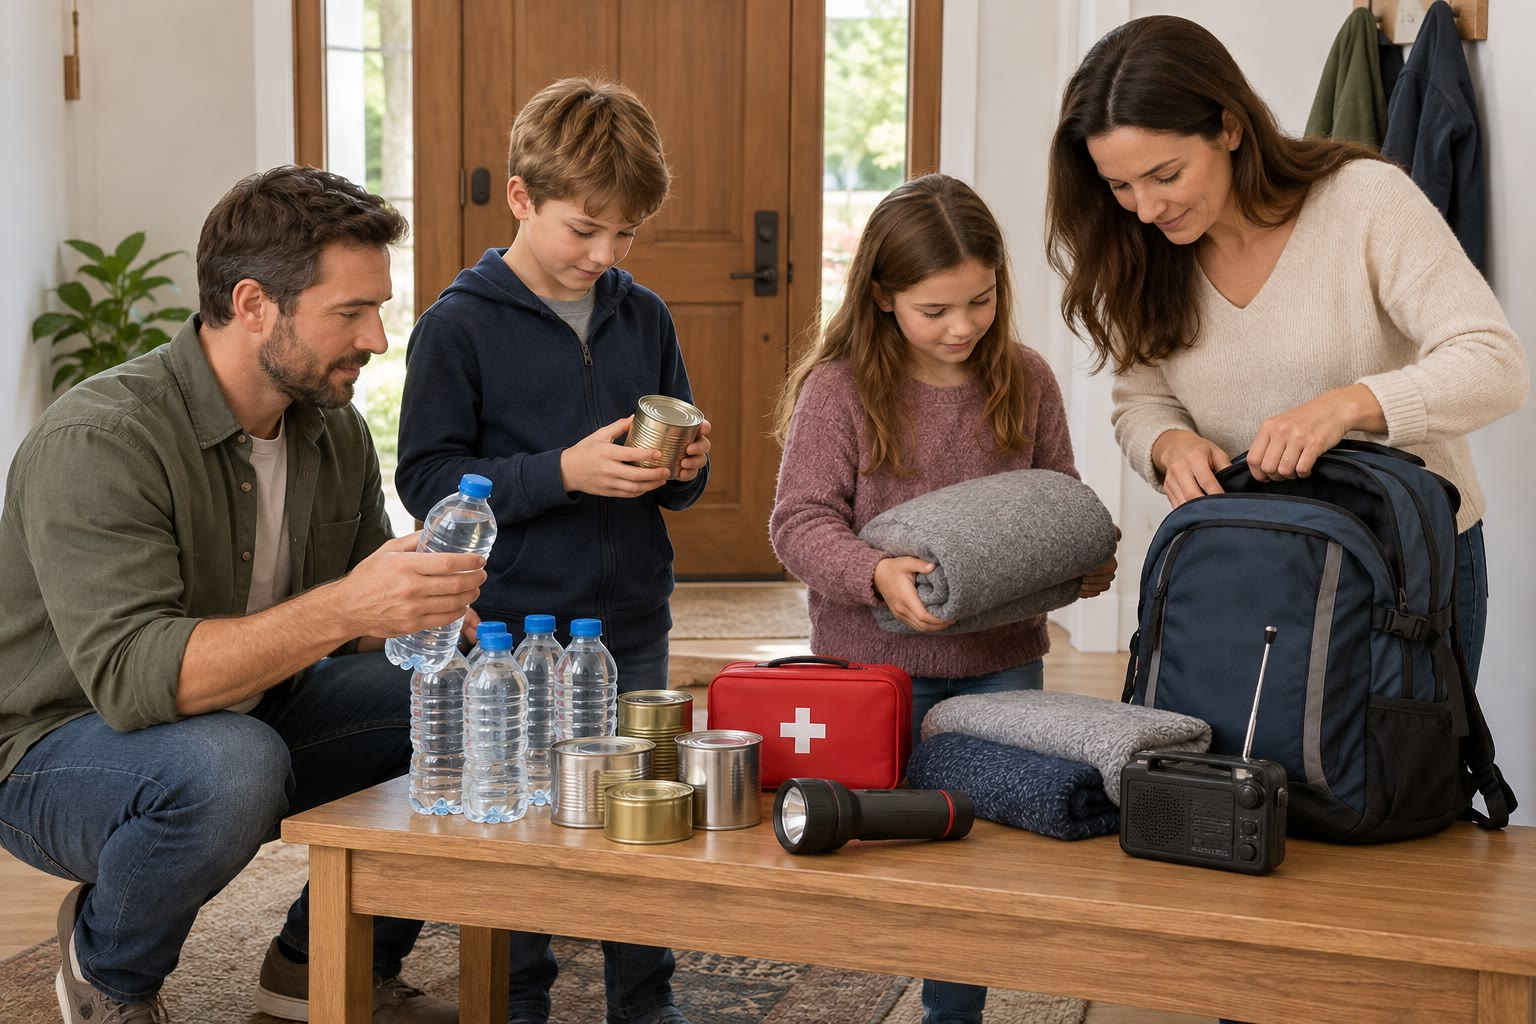
\includegraphics[width=\linewidth]{images/book1/ai/g9-emergency-kit.jpg}
\end{minipage}\hfill
\begin{minipage}[c]{0.52\linewidth}\raggedright
{\small الاستعداد: أسرة تتفقد حقيبة الطوارئ الخاصة بها، المحفوظة قرب الباب، جاهزة
لتؤخذ إذا اضطرت إلى المغادرة بسرعة: ماء وطعام يبقيان صالحين عدة أيام، ومصباح
يدوي، ومذياع يعمل دون كهرباء الشبكة، وبطاريات احتياطية، وحقيبة إسعافات أولية،
وبطانيات دافئة (رسم توضيحي مولَّد بالذكاء الاصطناعي لمشهد
عام).}
\end{minipage}
% ledger: ready:kit
\label{fig:g9:natural-risks:kit}
\end{omfigure}

\section{مراقبة البراكين والصدوع}

يراقب مرصد \omterm{def:g4:volcanoes-earthquakes-first-look:volcano}{البراكين} علامات الإنذار التي في \cref{ch:g7:volcanoes} بأجهزة تعمل
ليلًا ونهارًا وترسل قراءاتها إلى
المرصد.
% ledger: usgs:hvo-toolkit

\begin{omfigure}
\begin{tikzpicture}[x=1cm, y=1cm, font=\footnotesize, >={Stealth[length=2mm]}]
  % ground and cone
  \fill[black!13] (0,0) -- (0,1.0) -- (3.0,1.2) -- (5.4,3.6) -- (6.4,3.6) -- (8.8,1.2) -- (12,1.0) -- (12,0) -- cycle;
  \draw[black!60] (0,1.0) -- (3.0,1.2) -- (5.4,3.6) -- (6.4,3.6) -- (8.8,1.2) -- (12,1.0);
  % magma chamber and conduit
  \fill[omWarm!70] (5.9,0.6) ellipse (1.5 and 0.38);
  \fill[omWarm!70] (5.75,0.9) rectangle (6.05,3.6);
  \node[white, font=\scriptsize\bfseries] at (5.9,0.58) {الصهارة};
  % gas plume, drifting west
  \fill[black!10] (5.8,3.95) circle (0.3) (5.35,4.35) circle (0.4) (4.75,4.75) circle (0.45);
  % swollen east flank, dashed
  \draw[dashed, omWarm, line width=0.8pt] (6.45,3.7) .. controls (7.5,3.55) and (8.6,2.6) .. (8.85,1.25);
  \draw[->, omWarm] (7.3,2.75) -- (7.7,3.15);
  \node[anchor=west, align=left, text=omWarm!80!black] at (8.2,3.75) {الصهارة الصاعدة\\ تنفخ المنحدر};
  % tiltmeter on the east flank
  \fill[black] (7.75,2.12) rectangle (8.05,2.24);
  \draw[black!70] (8.1,2.2) -- (8.5,2.45);
  \node[anchor=west, align=left] at (8.5,2.55) {مقياس الميل: المنحدر\\ يميل حين ينتفخ};
  % GPS receiver on the west flank, and its satellite
  \draw[black, line width=0.6pt] (4.4,2.6) -- (4.4,2.95);
  \fill[black] (4.25,2.95) rectangle (4.55,3.05);
  \draw[black] (4.4,3.05) circle (0.1);
  \draw[black, fill=white] (1.7,4.85) rectangle (2.0,5.05);
  \draw[black] (1.4,4.95) -- (2.3,4.95);
  \node[anchor=east] at (1.35,4.95) {قمر صناعي};
  \draw[black!50, dashed] (4.3,3.15) -- (2.05,4.8);
  \draw[black!70] (3.05,2.65) -- (4.2,2.85);
  \node[anchor=east, align=right] at (3.0,2.6) {\foreignlanguage{arabic}{مستقبِل \babelsublr{GPS}: الأرض}\\ تتحرك\\ بالمليمترات};
  % gas instrument on the crater rim
  \fill[black] (6.45,3.6) rectangle (6.75,3.75);
  \draw[black!70] (6.8,3.75) -- (7.1,4.45);
  \node[anchor=west, align=left] at (7.1,4.6) {جهاز قياس الغازات: الغازات\\ المنبعثة من الفوهة};
  % seismometer (in the ground)
  \fill[black] (2.1,0.95) rectangle (2.4,1.1);
  \node[anchor=north, align=center] at (1.6,0.85) {مقياس الزلازل\\ زلازل صغيرة};
  % camera, east, looking at the summit
  \fill[black] (10.7,1.12) rectangle (11.0,1.32);
  \fill[black] (10.7,1.17) -- (10.55,1.12) -- (10.55,1.32) -- (10.7,1.27) -- cycle;
  \node[anchor=north, align=center] at (10.8,0.85) {آلة تصوير\\ تراقب القمة};
\end{tikzpicture}

{\small مراقبة \omterm{def:g4:volcanoes-earthquakes-first-look:volcano}{بركان} (رسم تخطيطي، ليس بمقياس رسم). ترصد \omterm{def:g7:earthquakes:seismometer}{مقاييس الزلازل} الهزات
الصغيرة؛ وتقيس مقاييس الميل ومستقبلات GPS، المثبتة في \omterm{def:g3:stones-pebbles-sand:rock}{الصخر}، كيف تميل الأرض
وتتحرك حين تتجمع \omterm{def:g7:volcanoes:magma}{الصهارة} تحتها؛ وتقيس أجهزة أخرى الغازات المنبعثة؛ وتراقب آلات
التصوير القمة. وتساعد \omterm{def:g4:clouds-rain-snow:rain-gauge}{مقاييس المطر} على تمييز إشارات \omterm{def:g4:volcanoes-earthquakes-first-look:volcano}{البركان} من آثار \omterm{def:g4:clouds-rain-snow:precipitation}{المطر}
الغزير.}
% ledger: usgs:hvo-toolkit
\label{fig:g9:natural-risks:monitoring}
\end{omfigure}

لا تعطي أي من هذه العلامات يوم \omterm{def:g4:volcanoes-earthquakes-first-look:eruption}{الثوران} وساعته. فالعلماء يقرؤونها معًا، كما يقرأ
الطبيب عدة قياسات لمريض، ويقولون كيف يتغير الخطر؛ والسلطات تقرر متى تغلق منطقة
ومتى تُجلي الناس. وفي بيناتوبو نجحت هذه السلسلة. أما في نيفادو ديل رويز، فقد كان
\omterm{def:g4:volcanoes-earthquakes-first-look:volcano}{البركان} يعطي علامات منذ سنة، بأسراب من \omterm{def:g4:volcanoes-earthquakes-first-look:earthquake}{الزلازل}، لكن الأجهزة كانت قليلة، والسلسلة
الممتدة من العلماء إلى سكان أرميرو كانت
مقطوعة.
% ledger: usgs:armero, usgs:hvo-toolkit, usgs:pinatubo-1991

وتُراقب الصدوع بالطريقة نفسها، بشبكات من \omterm{def:g7:earthquakes:seismometer}{مقاييس الزلازل} ومن محطات GPS تقيس،
مليمترًا بعد مليمتر، كيف يتحرك جانبا \omterm{def:g7:earthquakes:fault}{الصدع} ببطء. وهذا يبين أي الصدوع تختزن إجهاد
\omterm{def:g4:volcanoes-earthquakes-first-look:earthquake}{الزلزال} الكبير القادم، لكنه لا يبين متى سيأتي. وفي \omterm{def:g4:volcanoes-earthquakes-first-look:earthquake}{الزلازل}، تبقى \omterm{def:g9:natural-risks:prevention}{الوقاية} خط الدفاع
الأول.
% ledger: usgs:gps, usgs:eq-basics

\section{خرائط الأخطار ونطاقات الفيضان}

الخطوة الأولى في \omterm{def:g9:natural-risks:prevention}{الوقاية} هي معرفة أين يمكن أن يضرب الخطر.

\begin{definition}[خريطة الأخطار]\label{def:g9:natural-risks:hazard-map}
\emph{خريطة الأخطار}\index{خريطة الأخطار} تبين الأماكن التي يمكن أن يبلغها \omterm{def:g5:natural-hazards:hazard}{خطر
طبيعي}، وكثيرًا ما تميز عدة مستويات من الخطر. وتُرسم انطلاقًا مما فعله الخطر في
الماضي ومن شكل الأرض.
\end{definition}

\omterm{def:g2:drawing-to-map:map}{خريطة} نيفادو ديل رويز، في بداية هذا الفصل، \omterm{def:g2:drawing-to-map:map}{خريطة} أخطار: فالسيول الطينية في الماضي
كانت قد اتبعت \omterm{def:g1:landscapes-around-us:landform}{الأودية}، وستتبعها السيول القادمة أيضًا. وخرائط \omterm{def:g5:water-shapes-the-land:flood}{الفيضان} تقوم على
الفكرة نفسها. فالماء ينتشر على الأرض المنخفضة المستوية بجانب \omterm{def:g1:landscapes-around-us:water}{النهر}: وكلما ارتفع
\omterm{def:g5:water-shapes-the-land:flood}{الفيضان}، اتسع شريط الأرض الذي يغطيه. وترسم \omterm{def:g2:drawing-to-map:map}{خريطة} \omterm{def:g5:water-shapes-the-land:flood}{الفيضان} حد الماء \omterm{def:g5:water-shapes-the-land:flood}{لفيضان} مختار،
وكثيرًا ما يكون \omterm{def:g5:water-shapes-the-land:flood}{الفيضان} الذي فرصة بلوغه أو تجاوزه 1 من 100 في أي سنة. ويُسمى
\emph{\omterm{def:g5:water-shapes-the-land:flood}{فيضان} المئة عام}، لكنه ليس فيضانًا يأتي مرة كل قرن: فقد يأتي سنتين
متتاليتين.
% ledger: fema:flood-zones

\begin{omfigure}
\begin{tikzpicture}
\begin{axis}[axis equal image, xmin=3.5, xmax=7, ymin=2.7, ymax=5.5, width=11.5cm,
  enlargelimits=false, tick label style={font=\scriptsize}, xlabel={\foreignlanguage{arabic}{شرقًا \babelsublr{(km)}}},
  ylabel={\foreignlanguage{arabic}{شمالًا \babelsublr{(km)}}}, label style={font=\small}, xtick={3.5,4,...,7}, ytick={3,3.5,...,5.5},
  clip mode=individual]
\addplot[contour] table {figdata/out/grade-9-flood_zone-contours.dat};
\addplot[index contour] table {figdata/out/grade-9-flood_zone-index.dat};
\addplot[fill=omSea, draw=blue!40, line width=0.3pt] table {figdata/out/grade-9-flood_zone-zone10.dat} -- cycle;
\addplot[fill=blue!25, draw=blue!50, line width=0.3pt] table {figdata/out/grade-9-flood_zone-zone.dat} -- cycle;
\addplot[fill=blue!50, draw=none] table {figdata/out/grade-9-flood_zone-zone2.dat} -- cycle;
\addplot[only marks, mark=none, point meta=explicit symbolic, nodes near coords,
  nodes near coords align={center}, nodes near coords style={font=\tiny, fill=white, inner sep=0.6pt, text=omContour}]
  table[meta=z] {figdata/out/grade-9-flood_zone-index-lab.dat};
\addplot[river] table {figdata/out/grade-9-flood_zone-river.dat};
\end{axis}
\end{tikzpicture}

\smallskip
\begin{tikzpicture}[font=\footnotesize]
  \node[anchor=east] at (0,0.125) {ارتفاع الفيضان فوق النهر};
  \fill[blue!50] (0.2,0) rectangle (0.7,0.25); \node[anchor=west] at (0.8,0.125) {\qty{2}{m}};
  \fill[blue!25, draw=blue!50, line width=0.3pt] (1.9,0) rectangle (2.4,0.25); \node[anchor=west] at (2.5,0.125) {\qty{5}{m}};
  \fill[omSea, draw=blue!40, line width=0.3pt] (3.6,0) rectangle (4.1,0.25); \node[anchor=west] at (4.2,0.125) {\qty{10}{m}};
\end{tikzpicture}

{\small \omterm{def:g5:water-shapes-the-land:flood}{السهل الفيضي} \omterm{def:g1:landscapes-around-us:water}{لنهر} تلال فاردن، الذي يجري شرقًا. كل لون هو الأرض التي
يغطيها \omterm{def:g5:water-shapes-the-land:flood}{فيضان} لو ارتفع 2 أو 5 أو \qty{10}{m} فوق المستوى العادي \omterm{def:g1:landscapes-around-us:water}{للنهر}: وكل نطاق
يحتوي النطاقات الأصغر منه. وتبقى النطاقات ضيقة لأن جانبي \omterm{def:g1:landscapes-around-us:landform}{الوادي} يرتفعان بسرعة
من قاعه المستوي. والخطوط الرقيقة تصل بين نقاط على \omterm{def:g4:world-physical-map:altitude}{الارتفاع} نفسه، كل
\qty{10}{m}، مع عدد مكتوب كل \qty{50}{m}؛ ومثل هذه الخرائط هي موضوع
\cref{ch:g9:maps-of-the-earth}.}
% ledger: (invented region: figdata/grade-9/flood_zone.py, parts zone2, zone, zone10)
\label{fig:g9:natural-risks:flood-zones}
\end{omfigure}

\begin{method}[قراءة خريطة نطاقات الفيضان]
\begin{enumerate}
  \item جد \omterm{def:g5:water-shapes-the-land:flood}{الفيضان} الذي يمثله النطاق: كم يعلو فوق \omterm{def:g1:landscapes-around-us:water}{النهر}، أو كم مرة قد
        يأتي.
  \item حدد موقع المكان على \omterm{def:g2:drawing-to-map:map}{الخريطة}، \omterm{def:g2:drawing-to-map:scale}{بمقياس الرسم} أو بالشبكة.
  \item إذا وقع المكان داخل النطاق المظلل، فسيبلغه ذلك \omterm{def:g5:water-shapes-the-land:flood}{الفيضان}؛ وإذا وقع
        خارجه، فسيبقى جافًا في ذلك \omterm{def:g5:water-shapes-the-land:flood}{الفيضان}، لا في كل
        \omterm{def:g5:water-shapes-the-land:flood}{فيضان}.
  \item لمقارنة الأماكن، استعمل ارتفاعها فوق \omterm{def:g1:landscapes-around-us:water}{النهر}: فكلما كان أخفض،
        غمره \omterm{def:g5:water-shapes-the-land:flood}{الفيضان} أكثر.
\end{enumerate}
\end{method}

\begin{example}[ثلاثة بيوت بجانب النهر]
على \omterm{def:g2:drawing-to-map:map}{خريطة} كالتي أعلاه، يقوم بيت على أرض ترتفع \qty{3}{m} فوق \omterm{def:g1:landscapes-around-us:water}{النهر}. \omterm{def:g5:water-shapes-the-land:flood}{فالفيضان}
الذي يعلو \qty{2}{m} فوق \omterm{def:g1:landscapes-around-us:water}{النهر} لا يبلغه؛ أما فيضانا 5 و\qty{10}{m} فيبلغانه.
وبيت ثانٍ، على \omterm{def:g4:world-physical-map:altitude}{ارتفاع} \qty{8}{m} فوق \omterm{def:g1:landscapes-around-us:water}{النهر}، لا يبلغه إلا \omterm{def:g5:water-shapes-the-land:flood}{فيضان} \qty{10}{m}، وبيت
ثالث، على منحدر يرتفع \qty{30}{m} فوق \omterm{def:g1:landscapes-around-us:water}{النهر}، لا يبلغه أي من الثلاثة. فالبيت الأول
هو الأشد \omterm{def:g9:natural-risks:vulnerability}{هشاشة}: إذ تكفي لبلوغه \omterm{def:g5:water-shapes-the-land:flood}{فيضانات} أصغر، تأتي أكثر
تكرارًا.
\end{example}

\section{البناء لمقاومة الزلازل}

في \omterm{def:g4:volcanoes-earthquakes-first-look:earthquake}{الزلزال}، تتحرك الأرض ذهابًا وإيابًا تحت المبنى، فيهتز المبنى من أسفله؛ وفي
\omterm{def:g4:volcanoes-earthquakes-first-look:earthquake}{الزلزال} القوي، يأتي الخطر قبل كل شيء من المباني التي تتشقق وتسقط. ولا يستطيع
المهندسون إيقاف الاهتزاز، لكنهم يستطيعون البناء بحيث يحمل الهيكل قوى الاهتزاز
دون أن يسقط.
% ledger: iris:better-wall

\begin{omfigure}
\begin{tikzpicture}[x=1cm, y=1cm, font=\footnotesize, >={Stealth[length=2mm]}]
  % panel 1: a frame that leans
  \begin{scope}
    \fill[black!13] (-0.3,-0.25) rectangle (3.0,0);
    \draw[black!35, dashed] (0.2,0) rectangle (2.5,2.6);
    \draw[black, line width=1.2pt] (0.2,0) -- (0.75,2.6) -- (3.05,2.6) -- (2.5,0);
    \draw[black, line width=1.2pt] (0.47,1.3) -- (2.77,1.3);
    \draw[<->] (0.2,-0.45) -- (1.0,-0.45);
    \node[align=center, anchor=north] at (1.35,-0.65) {\foreignlanguage{arabic}{\textdir TRT(أ) هيكل عارٍ}\\ يميل وقد يسقط};
  \end{scope}
  % panel 2: braces
  \begin{scope}[xshift=3.7cm]
    \fill[black!13] (-0.3,-0.25) rectangle (3.0,0);
    \draw[black, line width=1.2pt] (0.2,0) rectangle (2.5,2.6);
    \draw[black, line width=1.2pt] (0.2,1.3) -- (2.5,1.3);
    \draw[omWarm, line width=1pt] (0.2,0) -- (2.5,1.3) (2.5,0) -- (0.2,1.3)
                                  (0.2,1.3) -- (2.5,2.6) (2.5,1.3) -- (0.2,2.6);
    \node[align=center, anchor=north] at (1.35,-0.65) {\foreignlanguage{arabic}{\textdir TRT(ب) دعامات قطرية}\\ تحفظ شكله};
  \end{scope}
  % panel 3: shear wall
  \begin{scope}[xshift=7.4cm]
    \fill[black!13] (-0.3,-0.25) rectangle (3.0,0);
    \draw[black, line width=1.2pt] (0.2,0) rectangle (2.5,2.6);
    \draw[black, line width=1.2pt] (0.2,1.3) -- (2.5,1.3);
    \fill[omWarm!35] (1.6,0) rectangle (2.5,2.6);
    \draw[black, line width=0.6pt] (1.6,0) rectangle (2.5,2.6);
    \node[align=center, anchor=north] at (1.35,-0.65) {\foreignlanguage{arabic}{\textdir TRT(ج) جدار قص صلب}\\ من الأعلى إلى الأسفل};
  \end{scope}
  % panel 4: base isolation
  \begin{scope}[xshift=11.1cm]
    \fill[black!13] (-0.3,-0.25) rectangle (3.0,0);
    \foreach \x in {0.35,1.35,2.35} \fill[omSea, draw=black!60, rounded corners=1pt] (\x-0.18,0) rectangle (\x+0.18,0.3);
    \draw[black, line width=1.2pt] (0.15,0.3) -- (2.55,0.3);
    \draw[black, line width=1.2pt] (0.2,0.3) rectangle (2.5,2.7);
    \draw[black, line width=1.2pt] (0.2,1.5) -- (2.5,1.5);
    \draw[<->] (0.2,-0.45) -- (1.0,-0.45);
    \node[align=center, anchor=north] at (1.35,-0.65) {\foreignlanguage{arabic}{\textdir TRT(د) عوازل تترك}\\ الأرض تتحرك تحته};
  \end{scope}
\end{tikzpicture}

{\small أربعة هياكل تهزها الأرض نفسها (رسم تخطيطي). الهيكل المؤلف من أعمدة وعوارض
وحدها يميل وقد ينهار (أ). والدعامات القطرية (ب) وجدران القص الصلبة (ج) تمنعه من
الميل؛ والوصلات المتينة بين العوارض والأعمدة تمسكه متماسكًا. والعوازل الموضوعة
تحت المبنى (د) تلين حين تتحرك الأرض، فلا يبلغ المبنى إلا جزء أصغر بكثير من
الحركة.}
% ledger: iris:better-wall, explo:base-isolation
\label{fig:g9:natural-risks:buildings}
\end{omfigure}

المبادئ نفسها تصلح لبيت أو مدرسة أو جسر. وأسهل ما يكون تطبيقها حين يُصمم المبنى،
لا حين تضاف إلى مبنى قديم بعد ذلك.

\begin{inthelab}[برج على صينية تهتز]
داخل البيت، ابنِ برجين صغيرين متساويين في الارتفاع من مصاصات الشرب أو العيدان
الخشبية والصلصال، على شكل هيكلين من طابقين. وأعطِ الثاني دعامات قطرية على كل
جوانبه. ضعهما على صينية، ثم حرّك الصينية بسرعة ذهابًا وإيابًا، برفق أولًا ثم بقوة
أكبر. أي البرجين يميل أولًا؟ وأيهما يحفظ شكله؟ ثم ضع البرج العاري على أربع كرات
زجاجية صغيرة تحت بطاقة خفيفة، وهزّ من جديد: ما الذي يتغير؟
\end{inthelab}

\section{الإنذار في الوقت المناسب}

آخر أجزاء \omterm{def:g9:natural-risks:prevention}{الوقاية} هو الإنذار. ففي حالة \omterm{def:g7:earthquakes:tsunami}{التسونامي}، يبدأ الإنذار في قاع \omterm{def:g2:water-on-earth:ocean}{المحيط}. ففي
مواقع قريبة من الأماكن التي بدأت فيها موجات \omterm{def:g7:earthquakes:tsunami}{تسونامي} مدمرة من قبل، يرقد على قاع
\omterm{def:g2:water-on-earth:ocean}{البحر} مسجّل ضغط يقرأ وزن الماء الذي فوقه كل \qty{15}{s}، وهذا يعطي ارتفاع سطح
\omterm{def:g2:water-on-earth:ocean}{البحر}. ويرسل قراءاته بالصوت عبر الماء إلى عوّامة مثبتة عند السطح، فتنقلها العوّامة
بالقمر الصناعي إلى مراكز الإنذار من \omterm{def:g7:earthquakes:tsunami}{التسونامي}. وارتفاع البحر بعيدًا عن أي \omterm{def:g1:landscapes-around-us:water}{ساحل}
يكشف عن \omterm{def:g7:earthquakes:tsunami}{تسونامي} في طريقه، قبل ساعات من بلوغه الشواطئ
البعيدة.
% ledger: ndbc:dart, nws:tsunami-speed

\begin{omfigure}
\begin{minipage}[c]{0.4\linewidth}\centering
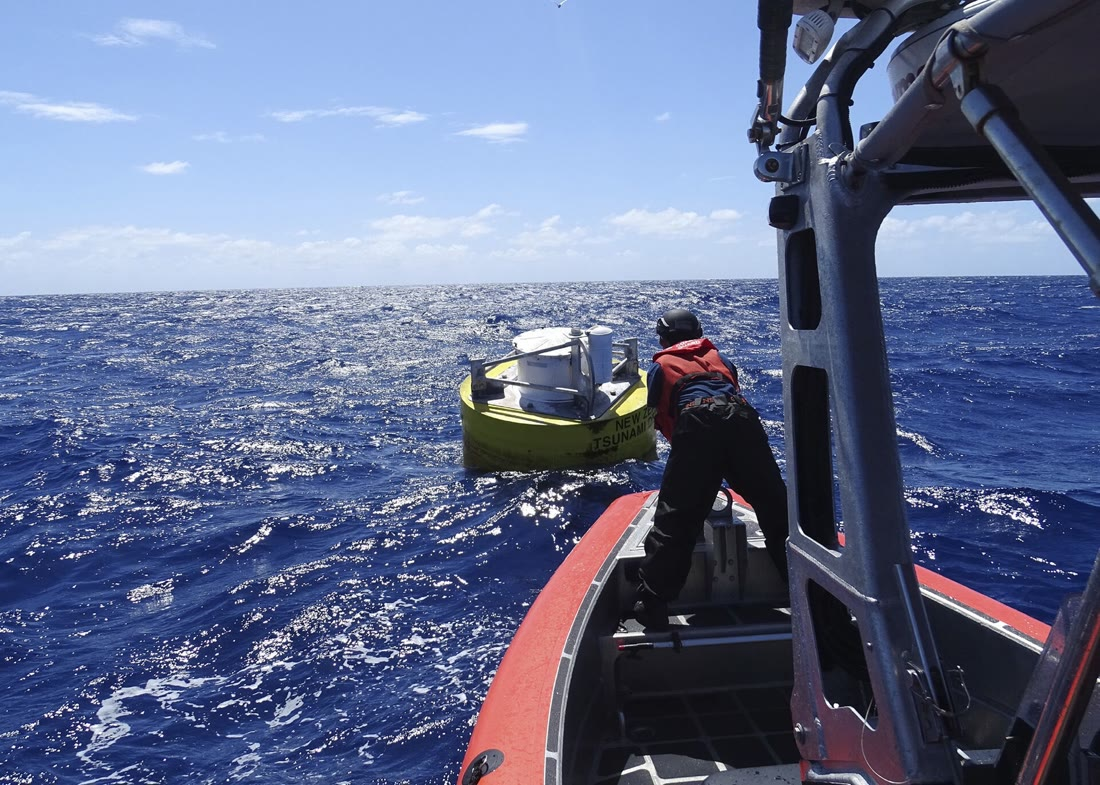
\includegraphics[width=\linewidth]{images/book1/g9-dart-buoy.jpg}
\end{minipage}\hfill
\begin{minipage}[c]{0.56\linewidth}\raggedright
{\small فرد من طاقم سفينة لخفر \omterm{def:g1:landscapes-around-us:water}{السواحل} الأمريكي يتفقد عوّامة إنذار من \omterm{def:g7:earthquakes:tsunami}{التسونامي} في
\omterm{def:g2:water-on-earth:ocean}{المحيط} الهادئ، في نوفمبر 2021. تطفو العوّامة فوق مسجّل ضغط على قاع \omterm{def:g2:water-on-earth:ocean}{البحر}، على
عمق آلاف الأمتار. خفر \omterm{def:g1:landscapes-around-us:water}{السواحل} الأمريكي (ملك عام، عبر ويكيميديا
كومنز).}
\end{minipage}
% ledger: commons:dart-buoy
\label{fig:g9:natural-risks:buoy}
\end{omfigure}

\begin{history}[شبكة من العوّامات]
في عام 2001 اكتملت أول مجموعة من ست محطات من هذا النوع، في \omterm{def:g2:water-on-earth:ocean}{المحيط} الهادئ. وبعد
\omterm{def:g7:earthquakes:tsunami}{تسونامي} ديسمبر 2004، الذي بلغ \omterm{def:g1:landscapes-around-us:water}{سواحل} \omterm{def:g2:water-on-earth:ocean}{المحيط} الهندي ولا نظام إنذار
فيها (\cref{ch:g7:earthquakes})، اتسعت الشبكة: ففي مارس 2008 كانت تضم 39
محطة.
\end{history}
% ledger: ndbc:dart

لا ينقذ الإنذار الأرواح إلا إذا بلغ أناسًا يعرفون ما يفعلون به: فطرق الوصول إلى أرض
أعلى معلَّمة ومجرَّبة، وحقيبة الطوارئ جاهزة، والمدارس تجري تدريبات. وفي أرميرو،
كان الخطر معروفًا \omterm{def:g2:drawing-to-map:map}{والخريطة} مرسومة؛ لكن الإنذار لم يبلغ البلدة
قط.
% ledger: ready:kit, usgs:armero

\section{تمارين}

\begin{exercise}[$\star$]\label{exo:g9:natural-risks:1}
خطر أم \omterm{def:g9:natural-risks:vulnerability}{هشاشة}؟ (أ) \omterm{def:g1:landscapes-around-us:water}{نهر} يفيض كل ربيع تقريبًا. (ب) قرية بلا نظام إنذار. (ج) بيوت
ثقيلة من الطوب بلا هيكل. (د) \omterm{def:g4:volcanoes-earthquakes-first-look:earthquake}{زلزال} قوي على \omterm{def:g7:earthquakes:fault}{صدع} قريب. (ه) بلدة مبنية عند مخرج
\omterm{def:g1:landscapes-around-us:landform}{وادٍ} جرت فيه سيول طينية من قبل.
\end{exercise}

\begin{exercise}[$\star$]\label{exo:g9:natural-risks:2}
صواب أم خطأ؟ صحّح الجمل الخاطئة. (أ) \omterm{def:g5:natural-hazards:hazard}{الخطر الطبيعي} في مكان لا يسكنه أحد \omterm{def:g9:natural-risks:risk}{مخاطر}
عالية. (ب) يمكن \omterm{def:g9:natural-risks:prevention}{للوقاية} أن تخفض \omterm{def:g9:natural-risks:vulnerability}{هشاشة} مدينة. (ج) تبين \omterm{def:g9:natural-risks:hazard-map}{خريطة الأخطار} أين يمكن أن
يضرب الخطر. (د) نظام الإنذار الجيد يجعل \omterm{def:g4:volcanoes-earthquakes-first-look:volcano}{البركان} أقل
خطرًا.
\end{exercise}

\begin{exercise}[$\star$]\label{exo:g9:natural-risks:3}
لكل خطر، قل هل يمكن التنبؤ به قبل أيام أو ساعات: (أ) \omterm{def:g5:natural-hazards:storm}{عاصفة}؛ (ب) \omterm{def:g5:water-shapes-the-land:flood}{فيضان} بعد \omterm{def:g4:clouds-rain-snow:precipitation}{مطر}
غزير؛ (ج) \omterm{def:g4:volcanoes-earthquakes-first-look:earthquake}{زلزال}؛ (د) وصول \omterm{def:g7:earthquakes:tsunami}{تسونامي} إلى \omterm{def:g1:landscapes-around-us:water}{ساحل} بعيد عن مكان
نشوئه.
\end{exercise}

\begin{exercise}[$\star$]\label{exo:g9:natural-risks:4}
% ledger: usgs:hvo-toolkit
استعمل رسم \omterm{def:g4:volcanoes-earthquakes-first-look:volcano}{البركان} المراقَب. ماذا يقيس كل جهاز، وأي علامة إنذار \omterm{def:g4:volcanoes-earthquakes-first-look:eruption}{بالثوران} يراقب؟
(أ) \omterm{def:g7:earthquakes:seismometer}{مقياس الزلازل}. (ب) مقياس الميل. (ج) مستقبِل GPS. (د) جهاز قياس
الغازات.
\end{exercise}

\begin{exercise}[$\star\star$]\label{exo:g9:natural-risks:5}
% ledger: usgs:armero
في عام 1985، بلغت السيول الطينية لنيفادو ديل رويز أرميرو، على بعد \qty{45}{km}،
بعد نحو ساعتين من \omterm{def:g4:volcanoes-earthquakes-first-look:eruption}{الثوران}. (أ) ما كان متوسط سرعتها، بالكيلومترات في الساعة؟
(ب) يمشي الإنسان بسرعة نحو \qty{4}{km/h}. فما المسافة التي كان يمكن للسكان أن
يمشوها في ساعتين؟ (ج) لماذا لم يغادروا؟ (د) اذكر أمرين كان يمكن أن
ينقذاهم.
\end{exercise}

\begin{exercise}[$\star\star$]\label{exo:g9:natural-risks:6}
% ledger: (invented region: figdata/grade-9/flood_zone.py)
استعمل \omterm{def:g2:drawing-to-map:map}{خريطة} نطاقات \omterm{def:g5:water-shapes-the-land:flood}{الفيضان} في تلال فاردن. (أ) أي \omterm{def:g5:water-shapes-the-land:flood}{فيضان} يغطي الشريط الأعرض؟
(ب) بشبكة \omterm{def:g2:drawing-to-map:map}{الخريطة}، قس عرض كل نطاق عبر \omterm{def:g1:landscapes-around-us:landform}{الوادي} عند \qty{5}{km} شرقًا. (ج) تقوم
حظيرة على أرض ترتفع \qty{6}{m} فوق \omterm{def:g1:landscapes-around-us:water}{النهر}. أي \omterm{def:g5:water-shapes-the-land:flood}{الفيضانات} الثلاثة يبلغها؟ (د) لماذا
يكون \omterm{def:g5:water-shapes-the-land:flood}{الفيضان} الذي يعلو \qty{2}{m} فوق \omterm{def:g1:landscapes-around-us:water}{النهر} هو الأكثر
تكرارًا؟
\end{exercise}

\begin{exercise}[$\star\star$]\label{exo:g9:natural-risks:7}
ضع كل حالة على شبكة \omterm{def:g9:natural-risks:risk}{المخاطر} (خطر منخفض أو مرتفع، \omterm{def:g9:natural-risks:vulnerability}{هشاشة} منخفضة أو مرتفعة)
وقل هل \omterm{def:g9:natural-risks:risk}{المخاطر} منخفضة أم متوسطة أم عالية. (أ) مبانٍ متينة وتدريبات في مدينة على
\omterm{def:g7:earthquakes:fault}{صدع} نشط. (ب) مخيم على \omterm{def:g5:water-shapes-the-land:flood}{السهل الفيضي} \omterm{def:g1:landscapes-around-us:water}{لنهر} نادرًا ما يفيض. (ج) قرية بيوتها ضعيفة
عند سفح \omterm{def:g4:volcanoes-earthquakes-first-look:volcano}{بركان} نشط، بلا مرصد. (د) مدينة على قمة تل بعيدة عن أي \omterm{def:g7:earthquakes:fault}{صدع} أو \omterm{def:g1:landscapes-around-us:water}{نهر} أو
\omterm{def:g4:volcanoes-earthquakes-first-look:volcano}{بركان}.
\end{exercise}

\begin{exercise}[$\star\star$]\label{exo:g9:natural-risks:8}
% ledger: iris:better-wall, explo:base-isolation
تُبنى ثلاث مدارس على الأرض نفسها. المدرسة A هيكل من أعمدة وعوارض بينها جدران من
الطوب؛ والمدرسة B لها الهيكل نفسه مع دعامات قطرية وجداري قص؛ والمدرسة C لها هيكل
B، قائمًا على عوازل. (أ) رتّبها من الأكثر أمانًا إلى الأقل أمانًا في \omterm{def:g4:volcanoes-earthquakes-first-look:earthquake}{الزلزال}.
(ب) اشرح ما تفعله الدعامات. (ج) اشرح ما تفعله
العوازل.
\end{exercise}

\begin{exercise}[$\star\star$]\label{exo:g9:natural-risks:9}
% ledger: fema:flood-zones
تبين \omterm{def:g2:drawing-to-map:map}{خريطة} \omterm{def:g5:water-shapes-the-land:flood}{الفيضانات} \omterm{def:g5:water-shapes-the-land:flood}{فيضان} المئة عام، الذي فرصة بلوغه أو تجاوزه 1 من 100 في أي سنة.
(أ) اكتب هذه الفرصة نسبة مئوية. (ب) يقول جار: «جاء \omterm{def:g5:water-shapes-the-land:flood}{فيضان} المئة عام في السنة
الماضية، فنحن في أمان مدة 99 سنة.» ما الخطأ؟ (ج) كم فيضانًا من هذا النوع يأتي
في المتوسط في 300 سنة؟
\end{exercise}

\begin{exercise}[$\star\star$]\label{exo:g9:natural-risks:10}
% ledger: ndbc:dart, nws:tsunami-speed
تقرأ محطة إنذار من \omterm{def:g7:earthquakes:tsunami}{التسونامي} ضغط قاع \omterm{def:g2:water-on-earth:ocean}{البحر} كل \qty{15}{s}. (أ) كم قراءة تُجري في
ساعة واحدة؟ (ب) وفي سنة من 365 يومًا؟ اكتب الجواب بالترميز العلمي. (ج) يعبر
\omterm{def:g7:earthquakes:tsunami}{التسونامي} \omterm{def:g2:water-on-earth:ocean}{المحيط} العميق بسرعة نحو \qty{800}{km/h}. فكم يستغرق ليبلغ ساحلًا على بعد
\qty{2400}{km}؟ (د) لماذا يهم هذا الزمن؟
\end{exercise}

\begin{exercise}[$\star\star\star$]\label{exo:g9:natural-risks:11}
% ledger: ready:kit
تُعد أسرة من أربعة أفراد حقيبة طوارئ فيها ماء يكفي 3 أيام، بمعدل نحو
\qty{3.8}{L} للشخص في اليوم، للشرب والاغتسال. (أ) كم لترًا من الماء تحتاج؟
(ب) كم قارورة سعتها \qty{1.5}{L} يساوي ذلك؟ (ج) سمِّ أربعة أشياء أخرى في الحقيبة،
وقل لماذا ينفع كل منها. (د) لماذا تُحفظ الحقيبة قرب الباب؟
\end{exercise}

\begin{exercise}[$\star\star\star$]\label{exo:g9:natural-risks:12}
% ledger: usgs:armero, usgs:hvo-toolkit
تقع مدينة بجانب \omterm{def:g1:landscapes-around-us:water}{نهر}، عند مخرج \omterm{def:g1:landscapes-around-us:landform}{وادٍ} ينحدر من \omterm{def:g4:volcanoes-earthquakes-first-look:volcano}{بركان} مكلل بالثلوج. وتحت شوارعها \omterm{def:g7:sediments-and-fossils:sediment}{رواسب}
سيول طينية قديمة. وقد بدأ \omterm{def:g4:volcanoes-earthquakes-first-look:volcano}{البركان} يهتز \omterm{def:g4:volcanoes-earthquakes-first-look:earthquake}{بزلازل} صغيرة. اكتب خطة \omterm{def:g9:natural-risks:prevention}{وقاية} من خمس نقاط
للمدينة. ولكل نقطة، قل هل تعمل على جانب الخطر (معرفة الخطر ومراقبته) أم على جانب
\omterm{def:g9:natural-risks:vulnerability}{الهشاشة} من \omterm{def:g9:natural-risks:risk}{المخاطر}.
\end{exercise}

\section{مسألة: أين تُبنى المدرسة الجديدة؟}

\begin{problem}[{مسألة نهاية الأسبوع --- تُوضع مدرسة جديدة على خريطة تلال فاردن،
بعيدًا عن الفيضانات والمنحدرات الشديدة والصدع؛ والجواب الأخير هو عدد البيوت داخل
نطاق الفيضان}]
\label{pb:g9:natural-risks:1}
% ledger: (invented region: figdata/grade-9/flood_zone.py: sites A, B, C; 17 of 28 houses in the 5 m zone)
تحتاج قرية تلال فاردن إلى مدرسة جديدة، وقد عُرضت ثلاثة مواقع: A وB وC، على \omterm{def:g2:drawing-to-map:map}{الخريطة}
أدناه. ونطاق \omterm{def:g5:water-shapes-the-land:flood}{الفيضان} المظلل على \omterm{def:g2:drawing-to-map:map}{الخريطة} هو كل الأرض التي ترتفع أقل من
\qty{5}{m} فوق \omterm{def:g1:landscapes-around-us:water}{النهر}، والتي يغطيها \omterm{def:g5:water-shapes-the-land:flood}{فيضان} كبير. ويعطي الجدول، لكل موقع، \omterm{def:g4:world-physical-map:altitude}{ارتفاع}
الأرض، ومستوى \omterm{def:g1:landscapes-around-us:water}{النهر} بجانبه، ومقدار ارتفاع الأرض على مسافة \qty{200}{m} مقيسة
أفقيًا عبر المنحدر.

\begin{center}
{\small
\begin{tabular}{|c|c|c|c|}
\hline
الموقع & \omterm{def:g4:world-physical-map:altitude}{ارتفاع} الأرض & مستوى \omterm{def:g1:landscapes-around-us:water}{النهر} بجانبه & ارتفاع الأرض على مسافة \qty{200}{m} \\
\hline
A & \qty{137}{m} & \qty{137}{m} & \qty{1.4}{m} \\
B & \qty{276}{m} & \qty{126}{m} & \qty{83}{m} \\
C & \qty{236}{m} & \qty{143}{m} & \qty{20}{m} \\
\hline
\end{tabular}}
\end{center}

\begin{omfigure}
\begin{tikzpicture}
\begin{axis}[axis equal image, xmin=3.5, xmax=7, ymin=2.7, ymax=5.5, width=11.5cm,
  enlargelimits=false, tick label style={font=\scriptsize}, xlabel={\foreignlanguage{arabic}{شرقًا \babelsublr{(km)}}},
  ylabel={\foreignlanguage{arabic}{شمالًا \babelsublr{(km)}}}, label style={font=\small}, xtick={3.5,4,...,7}, ytick={3,3.5,...,5.5}]
\addplot[contour] table {figdata/out/grade-9-flood_zone-contours.dat};
\addplot[index contour] table {figdata/out/grade-9-flood_zone-index.dat};
\addplot[fill=blue!25, draw=blue!50, line width=0.3pt] table {figdata/out/grade-9-flood_zone-zone.dat} -- cycle;
\addplot[only marks, mark=none, point meta=explicit symbolic, nodes near coords,
  nodes near coords align={center}, nodes near coords style={font=\tiny, fill=white, inner sep=0.6pt, text=omContour}]
  table[meta=z] {figdata/out/grade-9-flood_zone-index-lab.dat};
\addplot[river] table {figdata/out/grade-9-flood_zone-river.dat};
\addplot[fault] table {figdata/out/shared-region-fault.dat};
\addplot[only marks, mark=square*, mark size=1.5pt, mark options={fill=black}] table {figdata/out/grade-9-flood_zone-houses-in.dat};
\addplot[only marks, mark=square*, mark size=1.5pt, mark options={fill=black}] table {figdata/out/grade-9-flood_zone-houses-out.dat};
\addplot[only marks, mark=*, mark size=2.6pt, mark options={fill=omWarm, draw=black}, point meta=explicit symbolic,
  nodes near coords, nodes near coords align={anchor=south west},
  nodes near coords style={font=\small\bfseries, fill=white, inner sep=1pt, xshift=2.5pt, yshift=2.5pt}]
  table[meta=name] {figdata/out/grade-9-flood_zone-sites.dat};
\node[font=\footnotesize, fill=white, inner sep=1pt, anchor=west] at (axis cs:6.42,5.05) {صدع};
\coordinate (na) at (axis cs:3.7,4.75);
\fill[black] (axis cs:5.8,2.85) rectangle (axis cs:5.925,2.9);
\fill[white] (axis cs:5.925,2.85) rectangle (axis cs:6.05,2.9);
\fill[black] (axis cs:6.05,2.85) rectangle (axis cs:6.175,2.9);
\fill[white] (axis cs:6.175,2.85) rectangle (axis cs:6.3,2.9);
\draw[black, line width=0.4pt] (axis cs:5.8,2.85) rectangle (axis cs:6.3,2.9);
\node[font=\footnotesize, above, inner sep=1.5pt, fill=white] at (axis cs:6.05,2.9) {\qty{500}{m}};
\end{axis}
\fill[white, opacity=0.85] ($(na)+(-0.35,-0.1)$) rectangle ($(na)+(0.35,1.45)$);
\pic at (na) {northarrow};
\end{tikzpicture}

{\small القرية ومواقع المدرسة الثلاثة ونطاق \omterm{def:g5:water-shapes-the-land:flood}{الفيضان} (مظلل)، على \omterm{def:g2:drawing-to-map:map}{خريطة} تلال فاردن
(خطوط رقيقة متساوية \omterm{def:g4:world-physical-map:altitude}{الارتفاع} كل \qty{10}{m}). وكل مربع أسود صغير بيت. والخط الأسود
السميك \omterm{def:g7:earthquakes:fault}{صدع}.}
\label{fig:g9:natural-risks:school-map}
\end{omfigure}

\noindent\textbf{الجزء الأول --- نطاق الفيضان.}\par\nopagebreak
\begin{enumerate}[beginpenalty=10000]
  \item مستعينًا بمستويات \omterm{def:g1:landscapes-around-us:water}{النهر} في الجدول، قل في أي اتجاه يجري
        \omterm{def:g1:landscapes-around-us:water}{النهر}.
  \item احسب \omterm{def:g4:world-physical-map:altitude}{ارتفاع} كل موقع فوق \omterm{def:g1:landscapes-around-us:water}{النهر} الذي بجانبه.
  \item أي المواقع الثلاثة يقع في نطاق \omterm{def:g5:water-shapes-the-land:flood}{الفيضان}؟
  \item استعمل \omterm{def:g2:drawing-to-map:scale}{مقياس الرسم} لقياس عرض نطاق \omterm{def:g5:water-shapes-the-land:flood}{الفيضان}، عبر \omterm{def:g1:landscapes-around-us:landform}{الوادي}، عند
        الموقع A.
\end{enumerate}

\noindent\textbf{الجزء الثاني --- المنحدرات والصدع.}\par\nopagebreak
\begin{enumerate}[resume, beginpenalty=10000]
  \item الانحدار بالنسبة المئوية هو ارتفاع الأرض لكل \qty{100}{m} مقيسة
        أفقيًا. احسب الانحدار عند كل موقع.
  \item أي المواقع معرَّض \omterm{def:g5:natural-hazards:landslide}{لانزلاق أرضي}؟ علّل.
  \item استعمل \omterm{def:g2:drawing-to-map:scale}{مقياس الرسم} لتقدير المسافة من كل موقع إلى \omterm{def:g7:earthquakes:fault}{الصدع}.
  \item افترض أن \omterm{def:g7:earthquakes:fault}{الصدع} قد يتحرك من جديد. لماذا تكون الأرض الواقعة فوقه
        مباشرة مكانًا سيئًا لمدرسة؟
\end{enumerate}

\noindent\textbf{الجزء الثالث --- الاختيار.}\par\nopagebreak
\begin{enumerate}[resume, beginpenalty=10000]
  \item ارسم جدولًا فيه صف لكل موقع وثلاثة أعمدة: في نطاق \omterm{def:g5:water-shapes-the-land:flood}{الفيضان}؟
        منحدر شديد؟ على \omterm{def:g7:earthquakes:fault}{الصدع}؟ واملأه بنعم أو لا.
  \item أي موقع تختار؟ علّل اختيارك بالجدول.
  \item لا يزال الموقع المختار في منطقة قد تهتز فيها الأرض. اذكر طريقتين لبناء
        المدرسة، وعادة واحدة لتلاميذها، تخفض هشاشتها.
  \item ستكون المدرسة أيضًا ملجأً أثناء \omterm{def:g5:water-shapes-the-land:flood}{الفيضانات}. عُدّ بيوت القرية الواقعة داخل
        نطاق \omterm{def:g5:water-shapes-the-land:flood}{الفيضان}. ما الكسر الذي تمثله من مجموع
        البيوت؟
\end{enumerate}
\end{problem}
